%:Clase del documento
\documentclass[fontsize=10pt, Myfinal=true, twoside, numbers=noenddot]{scrbook}
%Minion=true, English=true, Myfinal=true

%:Paquete de estilos propuesto
\usepackage{cabeceras/libroETSI}

%:Paquete específico para cargar tikz (y sus librerías) y pgfplots
\usepackage{cabeceras/dtsc-creafig}

%:Paquete para notaciones específicas
\usepackage{cabeceras/notacion}

%:Paquete para incorporar aspectos concretos de la edición
\usepackage{cabeceras/edicionPFC}


%:Estas líneas de código son INNECESARIAS excepto para mostrar determinadas características en este manual. Pueden eliminarse o comentarse sin ningún problema.
%Se usan para compilar el capítulo estilolibroetsi.tex
\usepackage[final]{showexpl}
\lstset{explpreset={frame=none,rframe={}, numbers=none,numbersep=3pt, columns=flexible,language={[LaTeX]TeX},basicstyle=\ttfamily,keywordstyle=\color{blue}}}%numberstyle=\tiny,

%:Para modificar fácilmente la fuente del texto.
\makeatletter
\ifdtsc@Minion % Queremos utilizar la fuente Minion y lo hemos declarado al principio
	\ifluatex
		\setmainfont[Renderer=Basic, Ligatures=TeX,	% Fuente del texto 
		Scale=1.01,
		]{Minion Pro}
   		% En este caso conviene modificar ligeramente el tamaño de las fuentes matemáticas
		\DeclareMathSizes{10}{10.5}{7.35}{5.25}
		\DeclareMathSizes{10.95}{11.55}{8.08}{5.77}
		\DeclareMathSizes{12}{12.6}{8.82}{6.3}
%		\setmainfont[Renderer=Basic, Ligatures=TeX,	% Fuente del texto 
%		]{Adobe Garamond Pro}
%		\setmainfont[Renderer=Basic, Ligatures=TeX,	% Fuente del texto 
%		]{Palatino LT Std}
	\fi
\else
	\ifluatex
		% Para utilizar la fuente Times New Roman, o alguna otra que se tenga instalada
		\setmainfont[Renderer=Basic, Ligatures=TeX,	% Fuente del texto 
		Scale=1.0,
		]{Times New Roman}
	\else
		\usepackage{tgtermes} 	%clone of Times
		%\usepackage[default]{droidserif}
		%\usepackage{anttor} 	
	\fi
\fi
\makeatother

\usepackage[
    backend=biber,
    sorting=none, 
    %style=authoryear-icomp,
    %sortlocale=de_DE,
    %natbib=true,
    %url=false, 
    %doi=true,
    %eprint=false
]{biblatex}
\defbibheading{etsi}[]{%
        \chapter*{Bibliografía}%
        \chaptermark{Bibliografía} 
        \markboth{#1}{#1}}
\addbibresource{bibliografia.bib}

% Ejemplo de Glosario
\newacronym[type=main]{ETSI}{ETSI}{Escuela Técnica Superior de Ingeniería}
\newacronym[type=main]{US}{US}{Universidad de Sevilla}
\newacronym[type=main]{DMC}{DMC}{Canal Discreto sin Memoria}


\makeindex
\makeglossaries %Si no se quiere el glosario, comentar esta línea.

% Formato A4
\geometry
{paperheight=297mm,%
paperwidth=210mm,%
top=25mm,%
headsep=8.5mm,%
includefoot, 
textheight=240mm, 
textwidth=150mm, 
bindingoffset=0mm, 
twoside}

\usepackage[a4,center]{crop}%para poner las cruces de esquina de página, poner la opción cross

%:Esquema de numeración por defecto
\setenumerate[1]{label=\normalfont\bfseries{\arabic*.}, leftmargin=*, labelindent=\parindent}
\setenumerate[2]{label=\normalfont\bfseries{\alph*}), leftmargin=*}
\setenumerate[3]{label=\normalfont\bfseries{\roman*.}, leftmargin=*}
\setlist{itemsep=.1em}
\setlength{\parindent}{1.0 em}

\setcounter{tocdepth}{4}						% El nivel hasta el que se muestra el índice 

\usepackage{morewrites}
\usepackage[outputdir=build]{minted}
\setminted{fontsize=\footnotesize,linenos,breaklines,mathescape}
\usepackage[minted]{tcolorbox}
\tcbuselibrary{breakable,skins}

\newtcolorbox[auto counter,number within=chapter,list inside={qst}]{codigo}[2][]{,enhanced,breakable, left=1cm,colback=black!5!white,colframe=blue!0!black,fonttitle=\bfseries, title=Código ~\thetcbcounter: #2,#1}
\usepackage{adjustbox}
\usepackage{tikz-3dplot}
%\usepackage{subcaption}
\setcounter{secnumdepth}{40}

\usepackage{gensymb}

\usepackage{pdflscape}
\usepackage{multirow}
\usepackage{placeins}

\makeatletter
\providecommand\add@text{}
\newcommand\tagaddtext[1]{%
     \gdef\add@text{#1\gdef\add@text{}}}% 
     \renewcommand\tagform@[1]{%
          \maketag@@@{\llap{\add@text\quad}(\ignorespaces#1\unskip\@@italiccorr)}%
     }
\makeatother

\begin{document}
%:Para incluir toda la referencia bibliográfica aunque no se cite, descomente la siguiente línea
%\nocite{*}


%PORTADA
%ver edicionPFC.sty para modificaciones
%\mbox{pendiente}
%:Para crear la portada y la portada interior (pagina titular)
\titulo{Posicionamiento de un UAV usando \mbox{marcadores} visuales} %\mbox evita que se divida una palabra al cambiar de línea
\autor{Isidro Jesús Arias Sánchez}
\director{Manuel Vargas Villanueva}
\titulodirector{Profesor Titular}

\departamento{Dpto. de Ingeniería de Sistemas y Automática}
\centro{Escuela Técnica Superior de Ingeniería}
\universidad{Universidad de Sevilla}
\titulacion{Ingeniería Electrónica, Robótica y Automática}
\fecha{2020}
\nombretrabajo{Trabajo de Fin de Master} %Trabajo Fin de Grado, Proyecto fin de Máster,....

\hypersetup
	{
 	linkcolor=black, %Tocar para poner color en enlaces
	pdfauthor={\elautor},
	pdftitle={\nombretrabajo,\eltitulo}, 
	pdfkeywords={Latex, edición, formato de texto}	
	 }

%\portadaPFC{figuras/LogoUS.pdf}{figuras/LogoTSC.pdf} %logo de la Universidad y logo del departamento, si lo hubiera. Para cambiar el pie de página con los logos, debe editarse el fichero ediciónPFC.sty
\portadaPFC{figuras/LogoUS.pdf} %logo de la Universidad y logo del departamento, si lo hubiera. Para cambiar el pie de página con los logos, debe editarse el fichero ediciónPFC.sty

%Fin Portada

%:Todo lo que constituye la primera parte del libro que no es el cuerpo del libro en realidad
\frontmatter
\pagenumbering{Roman} %Pone la numeración en mayúscula (En español parece que es obligatorio)

%\include{dedicatoria/dedicatoria}%¿Comentar para proyectos/tesis?
% !TEX root =../LibroTipoETSI.tex
\chapter*{Agradecimientos}
%\pagestyle{especial}
\pagestyle{empty}
%\chaptermark{Agradecimientos}
\phantomsection
%\addcontentsline{toc}{listasf}{Agradecimientos}
%\vspace{1cm}
%{\huge{Agradecimientos}}
%\vspace{1cm}

\lettrine[lraise=-0.1, lines=2, loversize=0.25]{E}{stos} 4 años han sido mejores gracias al apoyo de algunas personas. Especialmente quiero agradecérselo a mis padres, Mercedes y José, a mi tía Antonia, a mi abuela Mercedes, a mi hermano Héctor, a Candi, mi novia, a mis amigos de Sevilla, Ángel, Carlos, David, Fernando, Jorge y Samuel, a los de Cádiz, Daniel, Juan Luís, Javier Mena, Javier Sanz, Pepe y Pedro, y por último y no menos importante, a mi tutores Manuel Vargas y Manuel Gil, y al resto de los profesores que me han sabido enseñar y de los que tanto he aprendido. Gracias a todos. 

{\flushleft{\hfill \emph{Isidro Arias Sánchez}}}%
\vspace{-.3cm}
%{\flushleft{\hfill \emph{Estudiante del Grado en Ingenieria Electrónica, Robótica y Mecatrónica}}}%
{\flushleft{\hfill \emph{Sevilla, 2019}}}%


%PFC/PFM/TESIS
% !TEX root =../LibroTipoETSI.tex
\chapter*{Resumen}
\pagestyle{especial}
\chaptermark{Resumen}
\phantomsection
\addcontentsline{toc}{listasf}{Resumen}

%\lettrine[lraise=-0.1, lines=2, loversize=0.2]{E}{n} este proyecto  se va a desarrollar el  estudio de  un vehículo aéreo no tripulado que tiene dos hélices o rotores orientables, denominado tiltrotor, del ingles \textit{tilt} que significa inclinar.

{\color{red} [Pendiente]}



\chapter*{Abstract}
\pagestyle{especial}
\chaptermark{Abstract}
\phantomsection
\addcontentsline{toc}{listasf}{Abstract}

%\lettrine[lraise=-0.1, lines=2, loversize=0.2]{T}{he} basis of this work is to contribute to the study of a convertible aerial vehicle in which the rotors, being tiltable, operate with the advantages of two different aircraft models, one of the helicopter type that gives it high maneuverability, and one of the airplane type that allows traveling long distances.

{\color{red} [Pendiente]}

 

% Índice abreviado 
% El índice abreviado se incluye también en algunos libros, con menor detalle que el completo. Descomentar las siguientes líneas.
\cleardoublepage
\phantomsection
\addcontentsline{toc}{listasf}{Índice Abreviado}
\pagestyle{especial}
\shorttoc{Índice Abreviado}{1}

%Índice normal, el completo
\cleardoublepage
\phantomsection
\pagestyle{especial}
\tableofcontents


\chapter*{\notationname}
\pagestyle{especial}
\chaptermark{\notationname}
\phantomsection
\addcontentsline{toc}{listasf}{\notationname}
\begin{longtable}{p{3cm}p{8.5cm}}
%TODO: Actualizar la notación de este trabajo
$\bm{P}$ & Posición del vehículo en ejes inerciales  \\
$\bm{V}$ & Velocidad del vehículo en ejes inerciales \\
$\bm{T}$ & Empuje aplicado en ejes cuerpo \\
$\bm{T_{rot}}$ & Empuje aplicado en ejes inerciales \\
$\theta$ &  Inclinación del quadrotor \\
$\bm{\tau}$ &  Par aplicado al quadrotor \\
$\omega$ & Medida del giróscopo \\
$\bm{a}$ & Medida del acelerómetro \\
$R^{UAV\rightarrow C\acute{a}mara}$  & Orientación del marcador vista desde el vehículo\\
$\bm{X}$ &  Vector de estados \\
\end{longtable}
\newpage

\chapter*{Acrónimos}
\pagestyle{especial}
\chaptermark{Acrónimos}
\phantomsection
\addcontentsline{toc}{listasf}{Acrónimos}
\begin{longtable}{p{3cm}p{8.5cm}}
$UAV$ & Vehículo aéreo no tripulado\\
$GCS$ & Estación de control terrestre \\
$NED$ & Ejes norte, este y abajo \\
\end{longtable}
\newpage

 %No incluir si no se quiere, comentándolo

%:Empieza el contenido del libro
\mainmatter

%:Página por defecto
\pagestyle{esitscCD}

\hypersetup
	{
 	linkcolor=blue, %Tocar para poner color en enlaces
	 }

%:Los diferentes capítulos, en carpetas separadas
%
% !TEX root =../LibroTipoETSI.tex
%El anterior comando permite compilar este documento llamando al documento raíz
\chapter{Introducción}\label{chp-02}

%\lettrine[lraise=-0.1, lines=2, loversize=0.2]{E}{n} la robótica, uno de los mayores problemas es la percepción del entorno y su ubicación en él. En concreto, cuando se habla de vehículos aéreos no tripulados (UAV), suelen poder posicionarse en el exterior con una precisión de metros. Sin embargo, cuando se trata de navegar en interiores o con precisión más alta el coste de los componentes puede ser muy elevados. Por ejemplo, en exteriores, se puede utilizar la \textit{navegación cinética satelital en tiempo real} (RTK) o en interiores se pueden utilizar balizas acústicas.


%%%%%%%%%%%%%%%%%%%%%%%
\lettrine[lraise=-0.1, lines=2, loversize=0.2]{A}{ctualmente}, los vehículos autónomos no están al alcance de cualquiera. Estos no deben de confundirse con los vehículos no tripulados, como los UAVs (Vehículos aéreos no tripulados) que si están más extendidos, llegando a utilizarse para ocio o para negocios estando al alcance del bosillo de cada vez más gente. La mayoría tienen una autonomía parcial y necesitan la supervisión de un piloto en algunas de sus fases de vuelo, como por ejemplo en el aterrizaje o cuando se navega cerca de obstáculos. Además muchos de ellos solo pueden volar en exteriores donde le llega la señal de los satélites. 
La causa de todas estás limitaciones está en que no pueden determinar dónde están ubicados con exactitud y que la precisión que sulelen tener es de varios metros. Si se mejorase ese aspecto, el número de aplicaciones en las que se podría utilizar sería enorme. 
Por ejemplo, se podría programar un vuelo de reconocimiento cuando se detecte un intruso en una propiedad. También perimitiría manipular objetos como la recogida y depósito de paquetes.  

% Autonomo permite:
% - que no tengan experiencia
% - que se pueda activar las 24 horas del día sin nadie pendiente
% - que sea escalable
% - Si existe una base es más inmediato
El interés de realizar estas tareas de forma autónoma no solo está en que cualquiera pueda hacer uso del vehículo, sin necesitar licencia ni habilidades especiales, si no que también hace el sistema más escalable. Si se quisiera por ejemplo, instalar un sistema de reparto de paquetes mediante vehículos aéreos, y la flota es cada vez más grande, llegará un momento que sea dificil que todos los pilotos se pongan de acuerdo compartiendo el mismo espácio aéreo. Si esta planificación la hace en su lugar un ordenador, posiblemente el sistema sea más optimo. Como última ventaja de la automatización se podría decir que el vehículo podría estar disponible de forma inmediata en cualquier momento y no obligaría a las personas a estar trabajando en horas de descanso. 

%Existen formas pero son más caras:
Si se disponen de los suficientes recursos existe la tecnología para conseguirlo, por ejemplo mediante balizas sonoras, que son usadas en interiores de fábricas o si se opera en el exterior, existe la posibilidad de  \textit{navegación cinética satelital en tiempo real} (RTK). Otra solución que no necesita de instalación en el entorno, son las cámaras o lídares, que con el uso de unos algoritmos llamados SLAM, pueden crear un mapa del entorno y ubicarse en él. El problema de estos es que o bien sus sensores son caros o bien tienen una alta carga computacional que obligan a instalar grandes y costosos ordenadores a bordo del vehículo. 

\begin{figure}[b]
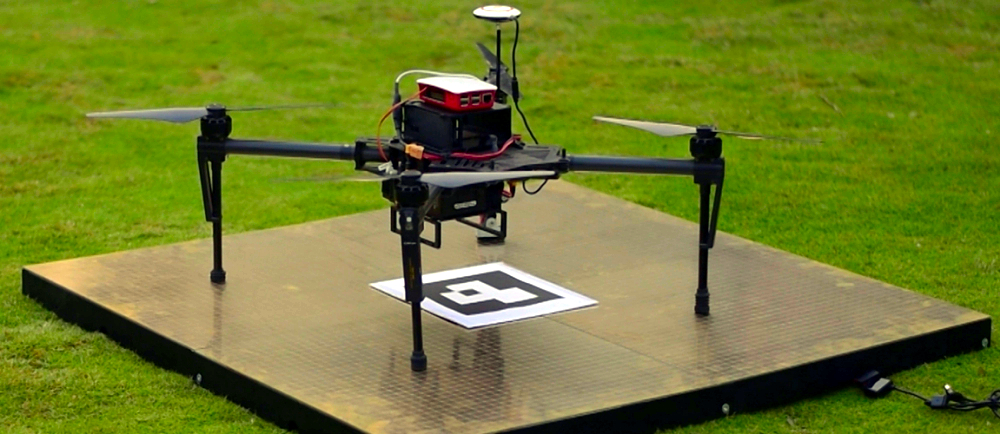
\includegraphics[width=0.7\textwidth]{introduccion/flytbase_en.jpg}
\caption{Estación de carga de \textit{Flytbase}}
\label{fig:flyt}
\end{figure}

%La alternativa: marcadores visuales
Lo que se busca en este trabajo es una alternativa más barata que consiga un posicionamiento centimétrico del vehículo. En concreto se ha hecho uso de unos marcadores visuales planos. Estos contienen figuras que son fácilmente detectables procesando una imagen de dicho marcador, por ejemplo los contornos de un cuadrilátero. Además, para su procesamiento se usará uno de los ordenadores embebidos más baratos del mercado 
% facil de imprimir, requiere menos computo, puede llegar a ser muy robusto. 
% Marcadores visuales. Solución robusta (no hay muchos falsos positivos) ya que es complicado encontrarse en el entorno algo parecido (no como los que usan una pelota), y además barata ya que tiene poco costo computacional, al contrario que los SLAM por ejemplo. 

 
% Implementaciones comerciales
Ya están a la venta algunas soluciones que utilizan esta tecnología para el aterrizaje automático. En concreto algunas  empresas como \textit{Everdrone} \cite{everdrone} y \textit{Flytbase} (ver figura \ref{fig:flyt}) ofrecen estaciones de carga con los mismos marcadores utilizados aquí. 

% Papers
Existen articulos en los que ya han utilizado marcadores visuales para mejorar el posicionamiento de un UAV, la mayoría teniendo como objetivo el aterrizaje automático. En \cite{sani2017automatic} se consigue que un quadrotor \textit{Parrot AR.Drone} aterrice sobre un marcador Aruco, incluso si brevemente se pierde la vista al marcador utilizando las medidas de la IMU. En \cite{yang2015precise} además de la IMU, se utiliza un sensor de flujo óptico para conseguir aterrizar el vehículo. En ninguno de los dos trabajos se utiliza un autopiloto de código abierto, sino se limitan a utilizar las interfaces de programación que aportan Parrot y DJI respectivamente para tomar las medidas de los sensores y comandarle una postura de referencia. 
Además, la falta de detalles de implementación que suele haber en este tipo de artículos, hace que su trabajo sea más dificil de ser repetido por el lector.
En este proyecto, lo que se quiere aportar otro enfoque en el que se hace uso del estimador de estados del autopiloto, el mismo que se utiliza para estimar la orientación y al que le llegan las medidas de la IMU, magnetómetro, barómetro, etc., para obtener una fuente precisa de posición.  
%Esa fusión de las medidas se realiza en el mismo autopiloto, y no en un ordenador externo, con la idea de que los retrasos en las comunicaciones tengan menor efecto. 

% Los puntos que se veran
En este trabajo en primer lugar, en el capítulo \ref{chp:est} se hace un estudio de una parte clave para el posicionamiento con marcadores, que es el estimador de estados. Además se elabora y se muestran los resultados de una simulación en la que se pone a prueba este. En el capítulo \ref{chp:pos} se explica cómo se ha implementado este posicionamiento, mostrando los componentes utilizados y explicando el programa creado. Finalmente, en ese mismo capítulo se enseñan los resultados experimentales a los que se ha llegado.  



\endinput

%\include{ControlDePX4/ControlDePX4}
%\include{ModeladoTiltrotor/ModeladoTiltrotor}
%\include{DisennoControl/DisennoControl}
%\include{SimulacionGazebo/SimulacionGazebo}
%\include{FabricacionTiltrotor/FabricacionTiltrotor}
%\chapter{Conclusiones} \label{chp-conclusiones}
%\lettrine[lraise=-0.1, lines=2, loversize=0.2]{S}{e} ha podido ver que el \textbf{autopiloto} \textit{PX4} ofrece una gran cantidad de funcionalidades, que vienen validadas por la multitud de vuelos que se realizan con este autopiloto. 


%- Manejo de medidadas retrasada es una idea intutitiva que no requiere de complejas demostraciones para saber que funcionarán.
%- Aun así se ha demostrado su eficacia en una simulación y se ha visto la mejora que conlleva.
%- Python como alternativa a matlab.	


Los resultados mostrados en este trabajo sirven sacar numerosas conclusiones. Par empezar, el \textbf{manejo de medidas retrasadas} aquí explicado es un método que no requiere de complejas demostraciones para entender que va a funcionar, ya que es intuitivo. Aun así, se ha probado en una simulación, la ventaja que supone tenerlo. Una simulación que se a programado en un lenguaje de programación abierto, que no tiene ningún coste económico, al contrario que el ampliamente usado \textit{Matlab}, y que además es de propósito más general. 



%- El uso de Arucos tiene una ventaja doble: barato y preciso 
%- Puede competir con métodos mucho más caros.
%- Si se quiere un vehículo completamente autónomo en todos los entornos, el mundo no a va estar lleno de balizas y marcadores. Por ahora lo más flexible es el SLAM, que podría ser asistido por estos marcadores.

%- La precisión de las medidas (verificadas de manera visual)
%- La utilidad del EKF
- La verificación del manejo de medidas retrasadas en un vuelo real
- La importacia de iterar rápidamente
- Es bueno para competir con las grander marcas

En cuanto al uso de \textbf{marcadores visuales para estimar la posición} claramente es una de las opciones más baratas para el posicionamiento, además de ser muy precisa. Por otro lado tiene una limitación importante de que allí donde navegue necesite que haya marcadores. Por muy baratos que sean imprimirlos, si se quiere un vehículo completamente autónomo en todos los entornos, no es factible llenar el mundo de marcadores o balizas.  
Sin embargo, estos podrían servir de apoyo a otras tecnologias que no necesitan ningún tipo de instalación fuera del vehículo.

Una de las ideas de este trabajo que no se ha visto en otros, es la de utilizar el estimador de estados del autopiloto para fusionar medidas de la visión. La ventaja que tiene esta es que reduce el efecto del retraso en las comunicaciones. Lo perjudicial es que si las medidas de la posición no son correctas pueden llegar a afectar en la estimación de la orientación del vehículo, ya que en un filtro de Kalman todos los estados pueden estar interelacionados. 



 





\chapter{Trabajos futuros}
%\lettrine[lraise=-0.1, lines=2, loversize=0.2]{L}{os} trabajos futuros vendrán marcados por la importante experiencia que me ha supuesto el desarrollo de este proyecto, tanto en la investigación y estudio de trabajos ya realizados, como en mi experimentación de prueba y error que me han ayudado en mi objetivo de llevar a buen puerto este Trabajo de Fin de Grado.
%A continuación, relaciono una serie de elementos y acciones  en los que me gustaría profundizar en futuros proyectos:


 
	\begin{itemize}
	\item Disminuir la necesidad de colocar marcadores cada poca distancia. Se podría usar lentes ojo de pez, varias cámaras (abajo y delante) o un gimbal.  
	\item Es verdad que colocar muchos marcadores puede ser no ser viable, pero por mucho que avanze la robótica siempre será mejor los marcadores artificiales a los naturales, para aquellas aplicaciones que se requieran una precisión extra.
	\item los marcadores visuales podrían tener diseños más bonitos
	\end{itemize}

	- Cuantificar la incertidumbre. Las medidas aportadas por este método es un caso en el que varía mucho su precisión, por ejemplo al alejarse
	- cámara en escala de grises? en realidad el grab no tarda mucho, pero la conversión desde el color no se cuanto tardará
	- Trasiciones con tramos con GPS o flujo óptico.
	- Aplicarle una derivada discreta la estimación de la visión e incluirla al filtro como una medida de velocidad
	- Tomar imagenes en un vuelo para crear un mapa en 2D . Especificación de waipoints clickando sobre el mapa.
	- Aprovechar la precisión de la posición para manipular objetos. Si no se generan muchas interferencias al magnetómetro se podría utilizar un imán.

\endinput


\begin{appendices}
\chapter{Simulador del estimador de estados}\label{chp:simu}

El siguiente archivo también puede verse y descargarse en el repositorio \url{https://github.com/isidroas/quadrotor\_simulator}

%\begin{codigo}{Simulador del estimador de estados  (\textit{main.py})}
\inputminted[bgcolor=black!5!white]{python}{apendices/quadrotor_simulator/main.py}
%\end{codigo} 

\chapter{Detector de marcadores visuales}

Los siguientes archivos se encuentran también en \url{https://github.com/isidroas/rpi\_vision\_uav}

\section{main.cpp}
\inputminted[bgcolor=black!5!white]{c++}{apendices/rpi_vision_uav/main.cpp}

\section{vision\_params.yml}\label{sec:vision-params}
\inputminted[bgcolor=black!5!white]{yaml}{apendices/rpi_vision_uav/vision_params.yml}

\section{marker\_vision.h}

\newcounter{lineInvertPoseA}
\newcounter{lineInvertPoseB}
\setcounter{lineInvertPoseB}{291}
\setcounter{lineInvertPoseA}{\thelineInvertPoseB -7}

\inputminted[bgcolor=black!5!white,lastline=\thelineInvertPoseA]{c++}{apendices/rpi_vision_uav/marker_vision.h}

La siguiente función invierte la posición y la rotación. También corrige la posición de la cámara con respecto al UAV. Sus argumentos son:
\begin{itemize}
\item rvec.  Vector de entrada. Vector de rotación del marcador con respecto a los ejes de la cámara
\item tvec.  Vector de entrada. Translación del marcador con respecto a los ejes de la cámara
\item pos.   Vector de salida. Posición del uav/cámara con respecto al marcador
\item eul.   Vector de salida. Orientación del uav con respecto al marcador. El orden de los elementos son 0: roll, 1: pitch, 2: yaw
\end{itemize}

\inputminted[bgcolor=black!5!white,firstline=\thelineInvertPoseB]{c++}{apendices/rpi_vision_uav/marker_vision.h}

\section{mavlink\_helper.h}
\inputminted[bgcolor=black!5!white]{c++}{apendices/rpi_vision_uav/mavlink_helper.h}
 
\end{appendices}

%:Empieza todo lo que no constituye el cuerpo en si del libro. Todo lo que va detrás
\backmatter

%:Indice de figuras, coméntese las siguientes líneas si no se desea
\cleardoublepage
\phantomsection

%:Para añadir una línea en blanco en el TOC y separar esta lista
\addtocontents{toc}{\protect\mbox{}\protect\hspace*{0pt}\par}
\addcontentsline{toc}{listasb}{\listfigurename}
\pagestyle{especial}
\listoffigures

%:Indice de tablas, coméntese las siguientes líneas si no se desea
\cleardoublepage
\phantomsection
\addcontentsline{toc}{listasb}{\listtablename}
\pagestyle{especial}
\listoftables

%:Indice de Programas
%\cleardoublepage
%\phantomsection
%\addcontentsline{toc}{listasb}{\lstlistlistingname}
%\pagestyle{especial}
%\lstlistoflistings

%:Bibliografía con biblatex y biber
\cleardoublepage
\phantomsection
\addcontentsline{toc}{listasb}{\bibname}
\pagestyle{especial}
%BIBER
\printbibliography[heading=etsi]

%:Índice alfabético de palabras
\cleardoublepage
\phantomsection
\addcontentsline{toc}{listasb}{\indexname}
\chaptermark{\indexname}
\printindex


%:Acrónimos
%\cleardoublepage
%\phantomsection
%\addcontentsline{toc}{listasb}{\glossaryname}
%\chaptermark{\glossaryname}
%\printglossaries

\end{document}
